\documentclass[11pt]{scrartcl}

    \usepackage{ucs}
    \usepackage[utf8]{inputenc}
    \usepackage[T1]{fontenc}
    \usepackage[ngerman]{babel}
    \usepackage{amsmath,amssymb,amstext}
    \usepackage{graphicx}
    \usepackage{parskip}
    \usepackage{hyperref}
    \usepackage{float}
    \usepackage{subfiles}
    \usepackage{titling}
    \usepackage{tabularx}
    \usepackage{ccicons}
    \usepackage{fontawesome}
    \usepackage{subfig}
    \usepackage[top=1in, bottom=1.25in, left=1.25in, right=1.25in]{geometry}
    \usepackage{xcolor}
    \usepackage{listings}
    \usepackage{enumerate}
    
    \lstset{basicstyle=\small,
      showstringspaces=false,
      commentstyle=\color{black},
      keywordstyle=\color{blue}
    }

    \graphicspath{{images/}{images/Antrieb/}{images/Fahrdaten}{images/Maschinentechnik}{images/Objekterkennung}{images/Stromversorgung}{images/Vision}}

        %\title{Dokumentation - PREN}
        \title{Testtat 2 - PREN}
        \author{A. Rebsamen, J. Grepper, M. Omlin, \\ M. Schöni, P. Marty, S. Ineichen}
        \date{\today{}, Luzern}

    \begin{document}

        \begin{titlingpage}
            \begin{center}
                \begin{Huge} %Exakter Modulnamen und Modulnamen ausgeschrieben
                    TA.BA{\_}PREN1.H1801 \\
                    \textbf{\thetitle} \\
                \end{Huge}
                \vspace{0.5cm}
                \begin{huge} %Author-Variable
                    \theauthor \\
                \end{huge}
                \vspace{0.5cm}
                \vspace{1cm}
                \begin{figure}[H] %Titelbild
                    \centering
                    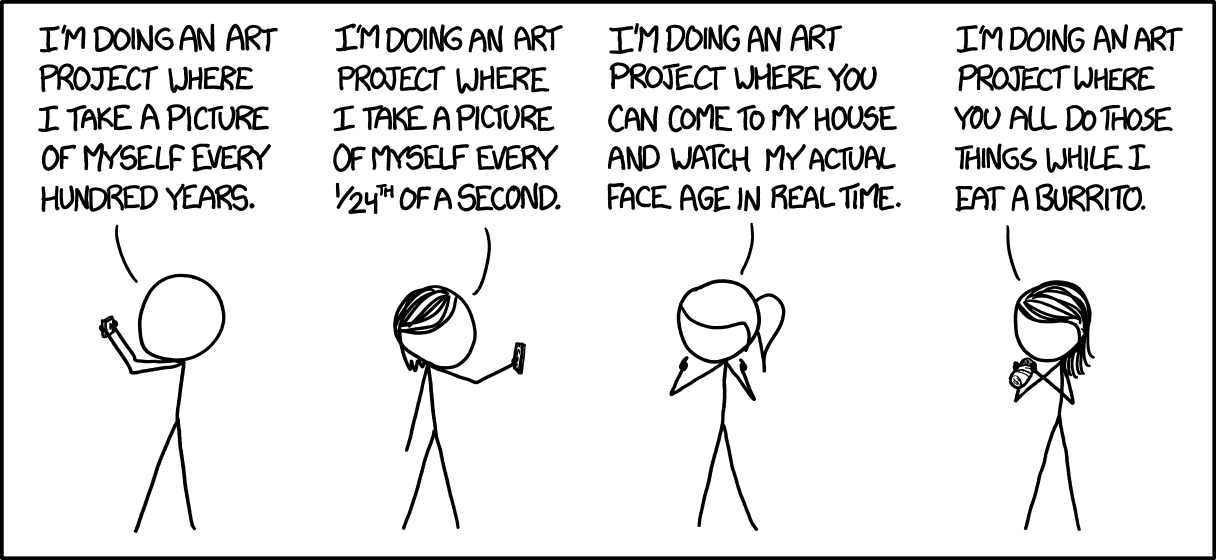
\includegraphics[width=0.6\textwidth]{images/comic.png}
                    \caption {https://xkcd.com/1496/}
                \end{figure}
                \vspace{0.5cm}
                \begin{huge} %Datumsvariable
                    \thedate
                \end{huge}
            \end{center}
        \end{titlingpage}

        %Inhaltsverzeichnis
        \tableofcontents
        \clearpage

        % \section{Anforderungs Analyse}
        % \subfile{sections/01_anforderungs_analyse/anforderungs_analyse.tex}
        % \clearpage

        % \section{Technologie Recherche}
        % \subfile{sections/02_technologie_recherche/technologie_recherche.tex}
        % \clearpage

<<<<<<< HEAD
        \section{Konzepte}
        \subfile{sections/03_konzepte/konzepte.tex}
        \subfile{sections/03_konzepte/Objekterkennung.tex}
        \clearpage
=======
       


        \section{Konzeptentscheid}
        Aufgrunde der in \ref{konzepte} beschriebenen Analysen wurden im Team zwei Gesamtkonzepte ausgewählt welche zur Realisierung weiter verfolgt werden. Dabei ist Plan-A (blau im Morphologischen Kasten) das primäre Konzept welches für die Konzeptentwicklung das Ziel für die Realisierung ist. Bei Problemen mit diesem Konzept ist Plan-B (rot im Morphologischen Kasten) als sekundäres Konzept zu betrachten. Sollte sich das Konzept Plan-A als zu schwierig, zu unzuverlässig oder allgemein als nicht gut genug herausstellen, kann das gesamte Konzept oder einzelne Komponente davon zu Plan B gewechselt werden.\\
        Für die Mehrheit der Komponente fiel der Entscheid für Plan-A auf die Option, welche in der Nutzwertanalyse mit dem grössten Gesamtnutzen bewertet wurde und für Plan-B mit dem zweitgrössten Gesamtnutzen. Abweichungen von der Nutzwertanalyse wurden im Team diskutiert und sind entsprechend in Kapitel \ref{konzepte} beschriebenen. 
>>>>>>> release/Testat2

        \vspace{1.5cm}

        \begin{flushleft}
        \begin{figure}[H]
            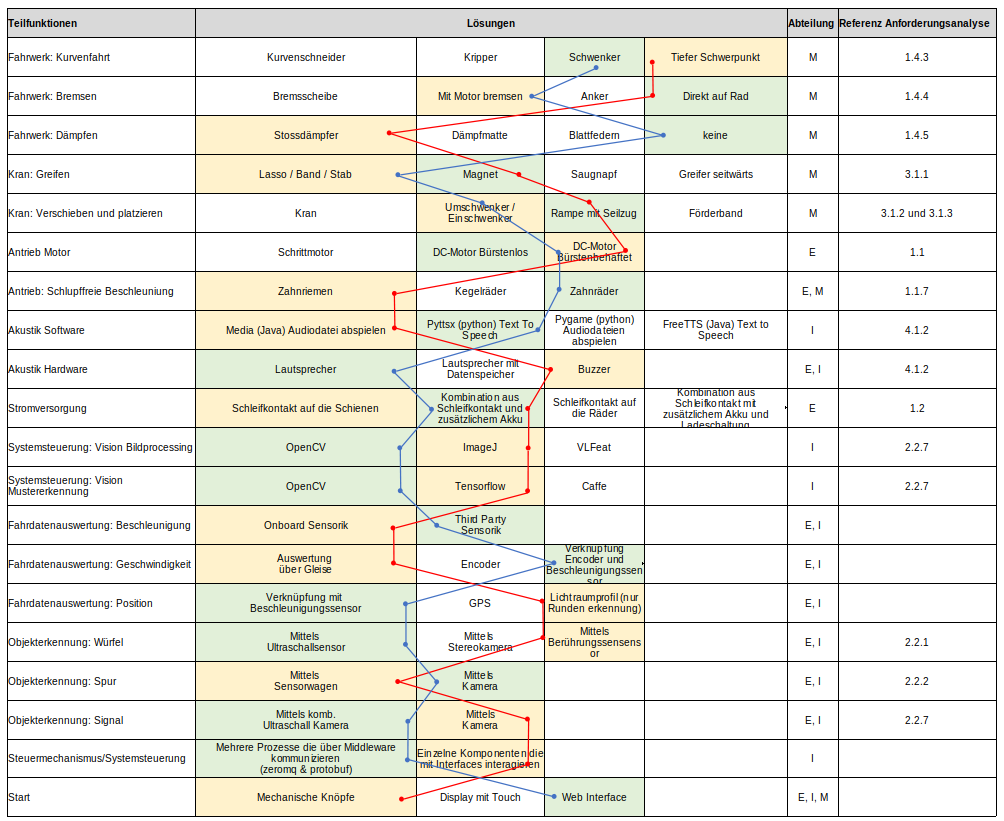
\includegraphics[width=1\textwidth]{morphologischer_Kasten.png}
            \caption{Morphologischer Kasten}
            \label{fig:morph}
        \end{figure}
        \end{flushleft}

        \pagebreak

        
       \pagebreak
        \section{Konzepte} \label{konzepte}
        \subfile{sections/03_konzepte/MT_Konzepte_master.tex}
        \clearpage
        \subfile{sections/03_konzepte/Antrieb.tex}
        \clearpage
        \subfile{sections/03_konzepte/Stromversorgung.tex}
        \clearpage
        \subfile{sections/03_konzepte/Fahrdaten.tex}
        \clearpage
        \subfile{sections/03_konzepte/Akustik.tex}
        \clearpage
        \subfile{sections/03_konzepte/Objekterkennung.tex}
        \clearpage
        \subfile{sections/03_konzepte/Vision.tex}
        \clearpage
        \subfile{sections/03_konzepte/SoftwareArchitekturKonzept.tex}
        \clearpage
        \subfile{sections/03_konzepte/CIKonzept.tex}
        \clearpage
    \end{document}